
\section{Experiments}
This section details both quantitative and qualitative evaluation of the system described in the previous sections. Due to the lack of animal keypoint datasets in the public domain, it is necessary to construct a new Benchmark Animal Dataset of Joint Annotations (BADJA). BADJA is a dataset comprising several video sequences with hand-clicked 2D joint labels and segmentation masks. Qualitative results are provided on BADJA and also on images used in the evaluation of 3D Menagerie (3DM). However, it should be noted this comparison is not entirely fair, since 3DM requires hand-clicked keypoints as input and system introduced in this chapter is optimized for video input.

\subsection{BADJA Dataset}
The BADJA dataset contains 9 videos, with manually collected keypoint and silhouette annotations. 7 video sequences were obtained from the DAVIS video segmentation dataset~\cite{Perazzi2016} and came with existing silhouettes, and the remainder were sourced from online stock footage. Segementation masks for these were generated using Adobe's UltraKey tool~\cite{adobe_ultrakey}. For all sequences, a set of 20 joints were labelled as illustrated in \figref{badja_examples}. The first 16 joints are located on legs, neck and tail, and defined by the rigged 3D SMAL skeleton. The final joints (nose tip, chin and ears) do not directly relate to 3D SMAL joints, but are instead defined by particular SMAL model vertices. A similar trick is used in SMALify~\cite{bogo16keep} to indicate the position of the human nose which has no corresponding SMPL joint. The collection of joints were chosen on the basis of being of informative to the skeleton and being simple for a non-expert human annotator to localize. To make manual annotation feasible and to ensure a diverse set of data, annotations are provided for every fifth video frame and were collected using the excellent LabelMe tool~\lazycite{LabelMe}{LabelMe}. 

The video sequences were selected to comprise a range of different quadrupeds undergoing various movement typical of their species. Although the dataset is perhaps insufficient in size to train deep neural networks, the variety in animal shape and pose renders it suitable for evaluating quadruped joint prediction methods. 

\subsection{Joint prediction}
\label{sec:exp-network}
%bjb_insert
For the joint predictor $\rho$ the stacked hourglass network~\cite{newell2016stacked} modified for multi-modal output is trained on synthetic animal silhouette data. Following state-of-the-art performance on related human 2D pose estimation datasets (\cite{andriluka14cvpr,lin2014microsoft}), the network consists of 8 stacks, 256 features and 1 block. Synthetic silhouette images of size $256\times 256$ are provided as input, which are obtained by randomly sampling shape and pose parameters from the SMAL model. The corresponding training targets are ground truth heatmaps produced by smoothing the 2D projected joint locations with a Gaussian kernel. As a benefit of working with synthetic data, training samples can be generated on the fly, which effectively results in a training set of infinite size. A small adaptation was required to prevent the network degenerating to an unfavourable solution on silhouette input: foreground masks were applied to both ground truth silhouette and predicted heatmaps to prevent the network degenerating to an all-zero heatmap, which produces a reasonably good loss and prevents the network training successfully. The network was trained using the RMSProp optimizer for 40k iterations with a batch size of 18 and learning rate of $2.5\times 10^{-4}$. The learning rate was decayed by 5\% every 10k iterations. Training until convergence took 24 hours on a Nvidia Titan X GPU.

Joint accuracy is evaluated with the Probability of Correct Keypoint (PCK) metric defined by Yang and Ramanan~\cite{yang2013articulated}. The PCK is the percentage of predicted keypoints which are within a threshold distance $d$ from the ground truth keypoint location. The threshold distance is given by $d=\alpha\sqrt{|S|}$ where $|S|$ is the area of the silhouette and $\alpha$ is a constant factor which we set to $\alpha=0.2$ for these experiments.

\figref{exp-network} shows a selection of maximum likelihood joint predictions on real world images. Note that despite being trained only on synthetic data, the network generalizes extremely well to animals in the wild. The performance extends even to species which were not present in the SMAL model, such as the impala and rhino. The network is also robust to challenging poses (\ref{fig:exp-network}b), occlusions (\ref{fig:exp-network}c) and distraction objects such as the human rider in (\ref{fig:exp-network}d). It is however susceptible to situations where the silhouette image is ambiguous, for example if the animal is facing directly towards or away from the camera. Figure~\ref{fig:blooper} contains examples of failure modes.

\begin{figure}[t]
\def\bb{\rule{2in}{0pt}\rule{0pt}{1in}}
\begin{center}
\resizebox{.95\linewidth}{!}{
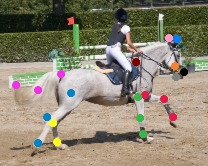
\includegraphics[width=.24\linewidth]{annotations/00110_rgb_horse_cropped.jpg}
~
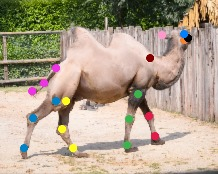
\includegraphics[width=.24\linewidth]{annotations/00021_camel_rgb_cropped.jpg}
~
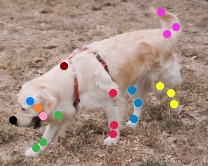
\includegraphics[width=.24\linewidth]{annotations/00085_rgb_dog_cropped.jpg}
~
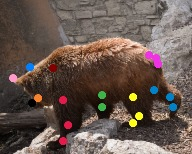
\includegraphics[width=.24\linewidth]{annotations/00008_bear_rgb_cropped.jpg}}
\end{center}
\caption{Example joint annotations from the BADJA dataset.  A total of 11 video sequences are in the dataset, annotated every 5 frames with 20 joint positions and visibility indicators.
}
\label{fig:badja_examples}
\end{figure}

    

\subsection{Optimal joint assignment}
Following non-maximum suppression of the joint heatmaps obtained in Section~\ref{sec:exp-network}, OJA is applied to select an optimal set of joints which initialize the final 3D model fitting stage. It can be seen that the OJA step is able to address many of the failure cases introduced by the joint prediction network, for example by eliminating physically implausible joint configurations (\figref{comparison}, row 1) or by resolving the ambiguity between the left and right legs (\figref{comparison}, row 2).  Table~\ref{tab:animal} summarizes the performance of both the raw network predictions and results of the two OJA methods. Over most of the sequences in the BADJA dataset it can be seen that the use of coverage terms (employed by the OJA-GA model) improves skeleton accuracy. In particular, the bear, camel and rs\_dog sequences show substantial improvements. The method does however struggle on the horsejump\_high sequence, in which part of the silhouette is occluded by the human rider which adversely affects the silhouette coverage term. Across all sequences the selected OJA-GA method improves joint prediction accuracy by 7\% compared to the raw network output. 

\begin{figure}[t]
\begin{floatrow}
\ffigbox{
\def\bb{\rule{2in}{0pt}\rule{0pt}{1in}}
\def\comparisonheight{20mm}
\begin{tabular}{ccc}
    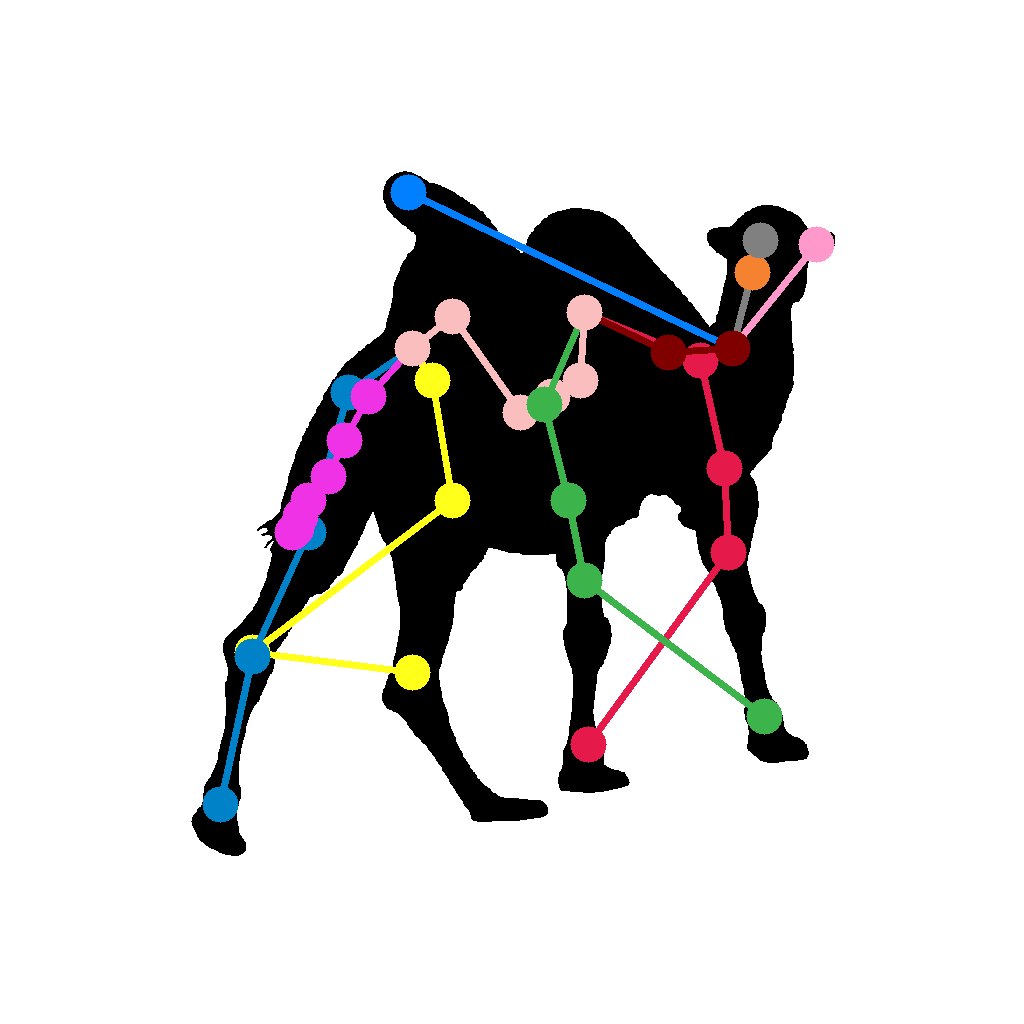
\includegraphics[trim={7cm 6cm 7cm 6cm},clip,height=\comparisonheight]{ga_vs_qp/0046_skel_sil_raw_2.png} &
    
    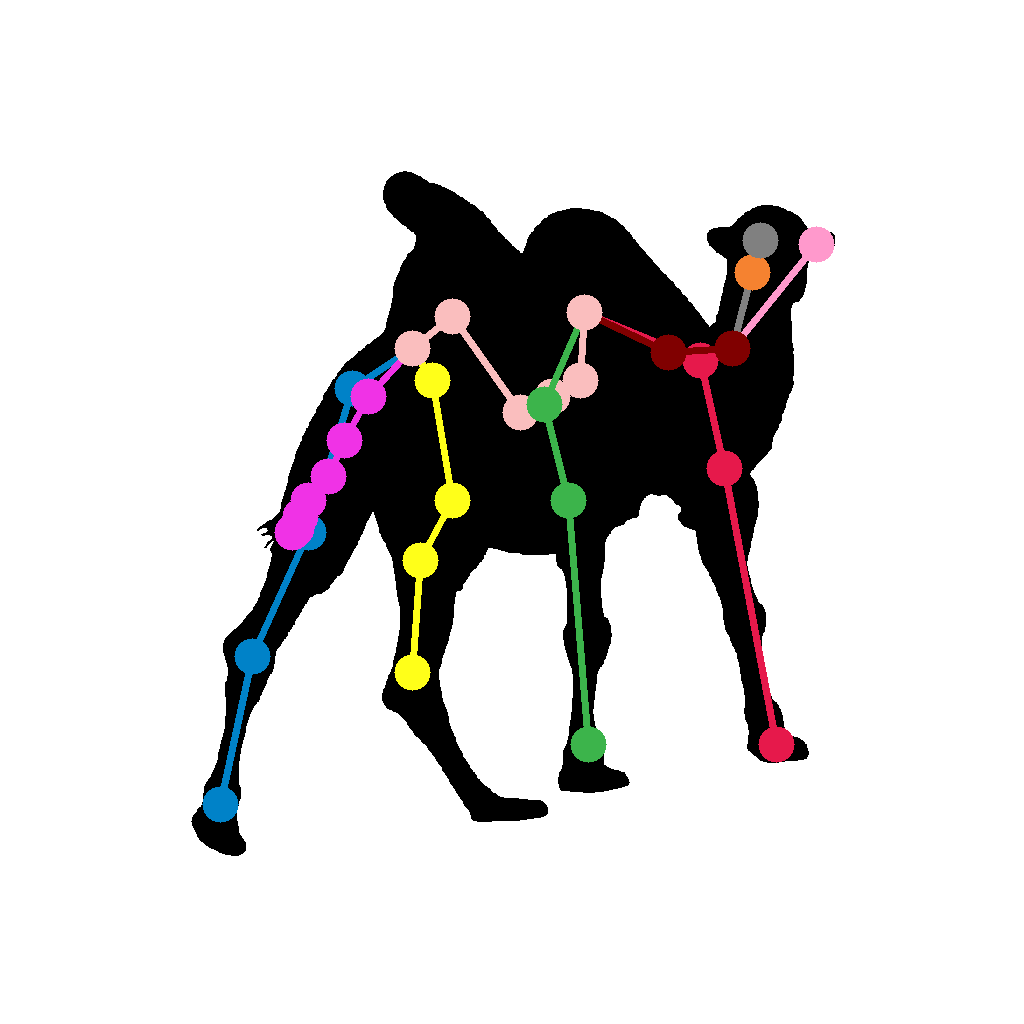
\includegraphics[trim={7cm 6cm 7cm 6cm},clip,height=\comparisonheight]{ga_vs_qp/0046_skel_sil_cleaned_qp_3.png} &
    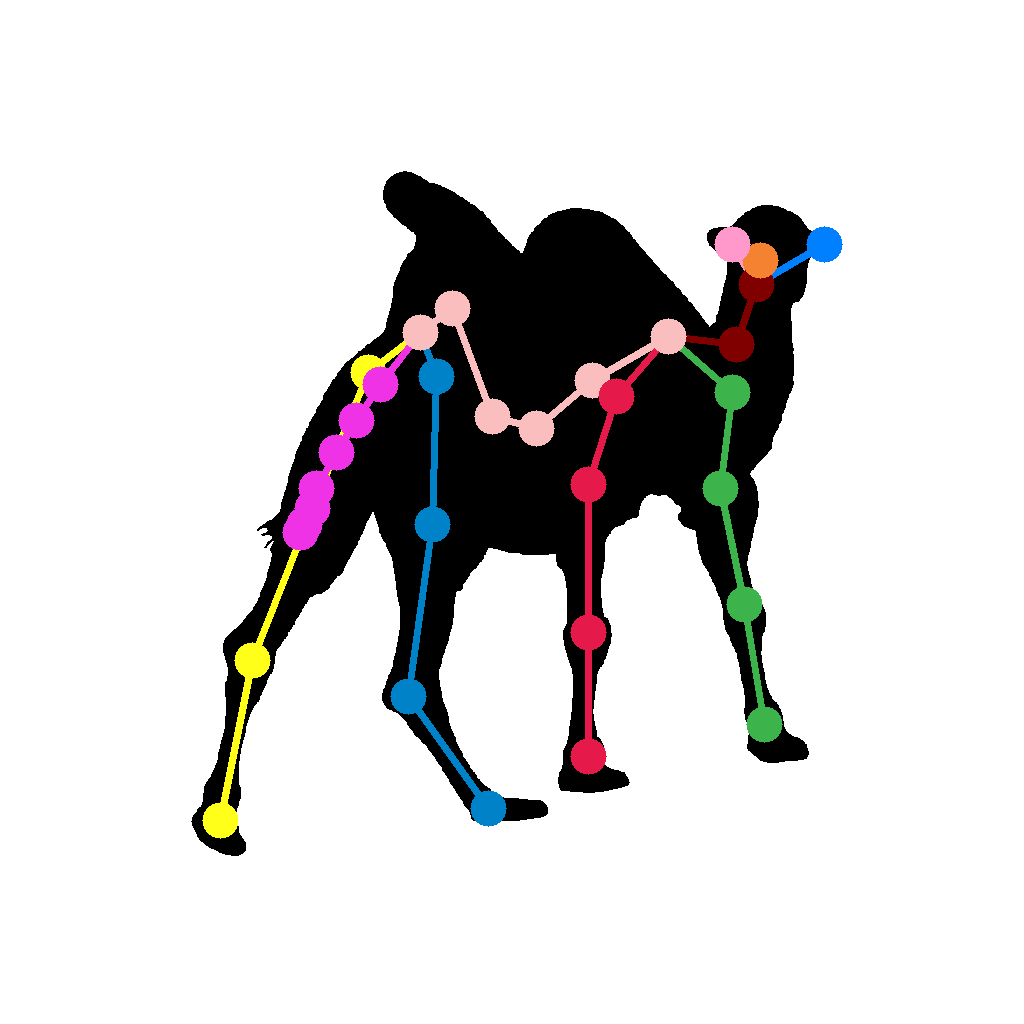
\includegraphics[trim={7cm 6cm 7cm 6cm},clip,height=\comparisonheight]{ga_vs_qp/0046_skel_sil_cleaned_ga_2.png} \\
    
    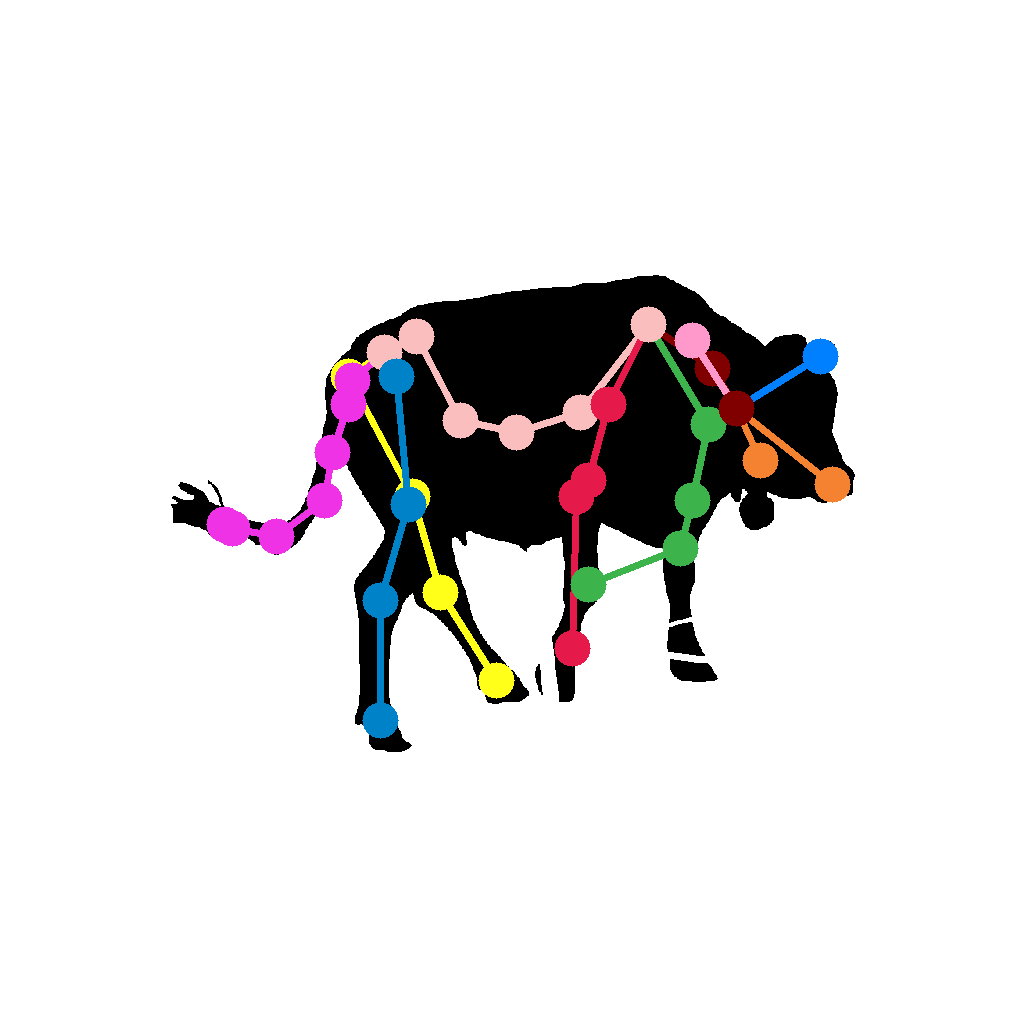
\includegraphics[trim={6cm 6cm 6cm 6cm},clip,height=\comparisonheight]{ga_vs_qp/0069_skel_sil_raw.png}
        &
    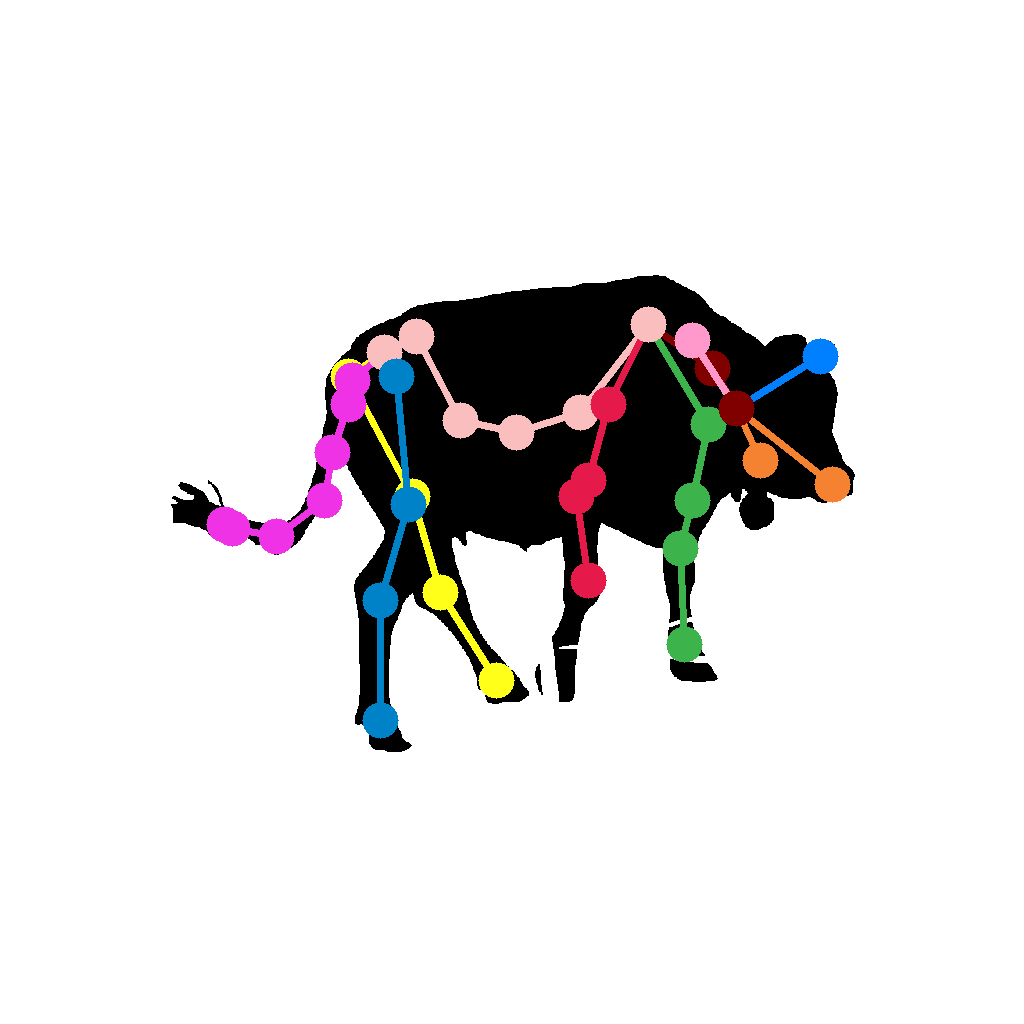
\includegraphics[trim={6cm 6cm 6cm 6cm},clip,height=\comparisonheight]{ga_vs_qp/0069_skel_sil_cleaned_qp.png}
        &
    {}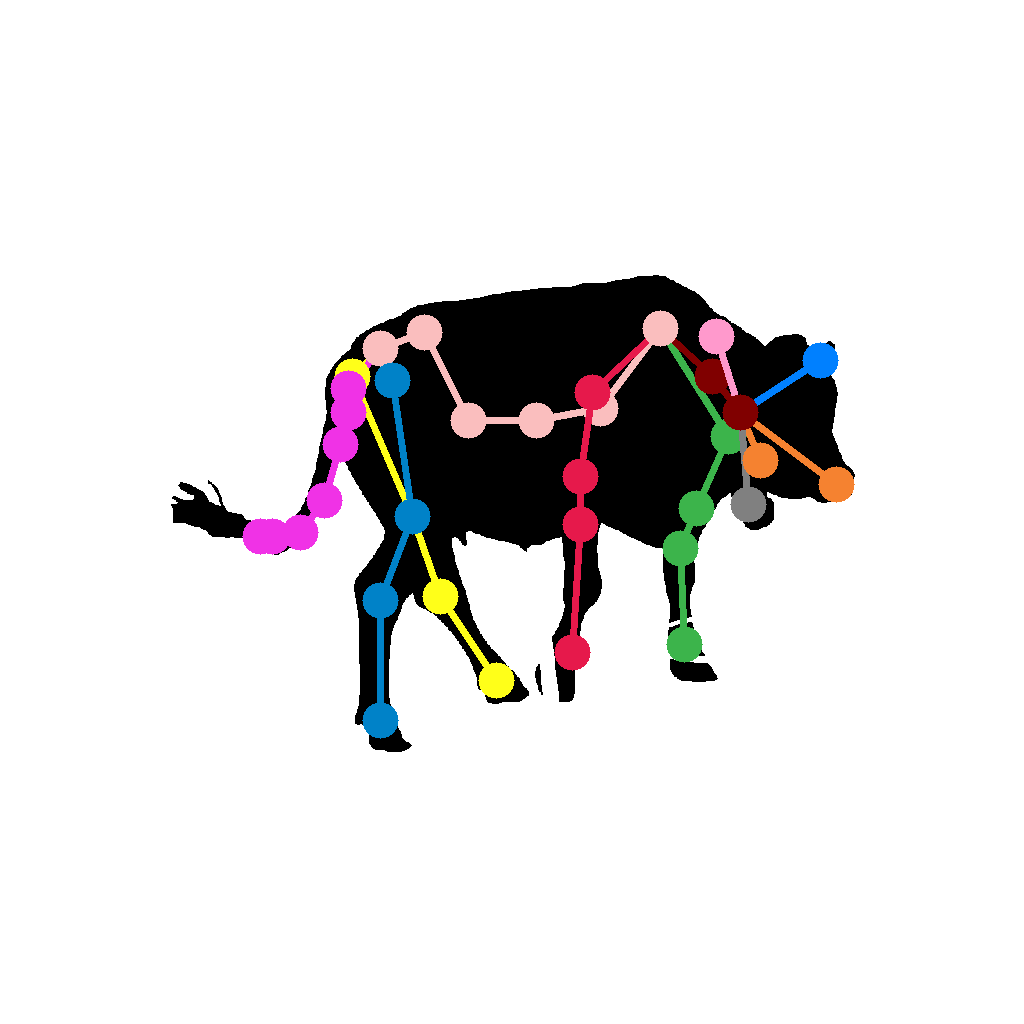
\includegraphics[trim={6cm 6cm 6cm 6cm},clip,height=\comparisonheight]{ga_vs_qp/0069_skel_sil_cleaned_ga.png} \\
    (a) & (b) & (c)
\end{tabular}
}{
\caption{Example skeletons from raw predictions (a), processed with OJA-QP (b), and OJA-GA (c).}
\label{fig:comparison}
}
~
\capbtabbox{%
\small
\begin{tabular}{lccc}
\toprule
                & Raw       & QP        & GA    \\
\midrule
bear           & 83.1      & 83.7      & \textbf{88.9}   \\
camel          & 73.3      & 74.1      & \textbf{87.1}   \\
cat            & 58.5      & \textbf{60.1}      & 58.4    \\
cows           & 89.2      & 88.4      & \textbf{94.7}  \\
dog            & \textbf{66.9}  & 66.6   & \textbf{66.9}  \\
horsejump-high & 26.5      & \textbf{27.7}      & 24.4   \\
horsejump-low  & 26.9      & 27.0      & \textbf{31.9}   \\
tiger          & 76.5      & 88.8      & \textbf{92.3}   \\
rs\_dog        & 64.2      & 63.4      & \textbf{81.2}   \\
\midrule
Average        & 62.8      & 64.4      & \textbf{69.5}   \\
\bottomrule
\end{tabular}
}{\caption{Accuracy of OJA on BADJA test sequences.}
\label{tab:animal}
}
\end{floatrow}
\end{figure}

\begin{table}[ht]
\centering
\small
\begin{tabular}{@{}cccccccccc@{}}

\toprule
        \multirow{2}{*}{Seq.}  & \multirow{2}{*}{Family} & \multicolumn{2}{c}{PCK (\%)} &   \multirow{2}{*}{Mesh}  & \multirow{2}{*}{Seq.} & \multirow{2}{*}{Family} & \multicolumn{2}{c}{PCK (\%)} &   \multirow{2}{*}{Mesh} \\
&  & Raw                  & OJA-GA &  &&& Raw                  & OJA-GA           \\ \midrule
01 & Felidae         & 91.8     & 91.9  & 38.2   &  06 & Equidae         & 84.4     & 84.8  & 19.2     \\
02 & Felidae         & 94.7     & 95.0  & 42.4   &  07 & Bovidae         & 94.6     & 95.0  & 40.6     \\
03 & Canidae         & 87.7     & 88.0  & 27.3   &  08 & Bovidae        & 85.2     & 85.8  & 41.5     \\  
04 & Canidae         & 87.1     & 87.4  & 22.9   &  09 & Hippopotamidae  & 90.5     & 90.6  & 11.8     \\
05 & Equidae         & 88.9     & 89.8  & 51.6   &  10 & Hippopotamidae  & 93.7     & 93.9  & 23.8     \\    
\bottomrule
\end{tabular}%

\caption{Quantitative evaluation on synthetic test sequences. The performance of the raw network outputs and OJA methods are evaluated using the probability of correct keypoint (PCK) metric. Mesh fitting accuracy is evaluated by computing the mean distance between the predicted and ground truth vertices.}
\label{tab:synthetic}
\end{table}


\begin{figure}[t]
\def\bb{\rule{2in}{0pt}\rule{0pt}{1in}}
\def\bjb{\rule{0.5in}{0pt}\rule{0pt}{0.25in}}
\setlength{\fboxsep}{0pt}%
\centering
\begin{tabular}{ccc}
\includegraphics[width=0.3\linewidth]{smal_comp_cat/rgb_cropped.jpg}
&
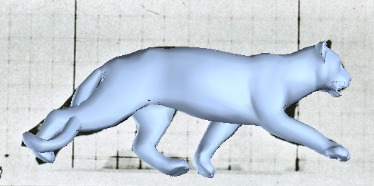
\includegraphics[width=0.3\linewidth]{smal_comp_cat/muybridge_107_smal_res_cropped.jpg}
&
\includegraphics[width=0.3\linewidth]{smal_comp_cat/3d_fit_overlay_rgb_cropped.jpg}
\\

\includegraphics[width=0.3\linewidth]{smal_comp_horse/rgb_cropped.jpg} &
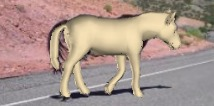
\includegraphics[width=0.3\linewidth]{smal_comp_horse/00049424_ferrari_smal_cropped.jpg} &

\includegraphics[width=0.3\linewidth]{smal_comp_horse/3d_fit_overlay_rgb_cropped.jpg} \\

RGB & SMAL \cite{zuffi2017menagerie} & \textbf{Ours}
\end{tabular}
\caption{Results are comparable in quality to SMAL~\cite{zuffi2017menagerie}, but note that we do not require hand-clicked keypoints.
}
\label{fig:compar_smal}
\end{figure}
    

\subsection{Model fitting}
The predicted joint positions and silhouette are input to the 3D model fitting optimization phase, which proceeds in four stages. The first stage solves for the model's global rotation and translation parameters, which positions the camera. Following SMPLify~\cite{bogo16keep}, this camera stage is solved for torso points only, which remain largely fixed through shape and pose variation. The remaining stages solve for all shape, pose and translation parameters the emphasis of the priors gradually decreased. The silhouette term is introduced in the penultimate stage, as including this too early can lead to the optimizer finding unsatisfactory local minima.

The final outputs of our optimization pipeline are shown in \figref{example_results}. In each of the cases illustrated the optimizer is able to successfully find a set of pose and shape parameters which, when rendered, closely resembles the input image. The final row of \figref{example_results} demonstrates the generalizability of the proposed method: the algorithm is able to find a reasonable pose despite no camel figurines being included in the original SMAL model.

\subsubsection*{Comparison to other work.} Our approach is compared visually to that given by Zuffi {\em et al.}~\cite{zuffi2017menagerie}. Recall that their results require hand-clicked keypoints rather than fitting to points predicted automatically by the hourglass network, which was trained on synthetic animal images. Further, their work is optimized for single frame fitting and is tested on animals in simple poses, whereas the focus of this work is on the more challenging task of tracking animals in video. \figref{compar_smal} shows the application of our model to a number of single frame examples from the SMAL result data~\cite{zuffi2017menagerie}.

\subsubsection*{Quantitative experiments.}
There is no existing ground truth dataset for comparing reconstructed 3D animal meshes, but an estimate of quantitative error is obtained by testing on synthetic sequences for a range of quadruped species. These are generated by randomly deforming the model and varying the camera position to animate animal motion, see Figure~\ref{fig:synth}. Table~\ref{tab:synthetic} shows results on these sequences. 
%bjb_insert

\begin{figure}[t!]
\begin{tabular}{cccccc}
\includegraphics[width=0.16\linewidth]{synth_pipeline_45/gt_fit_cropped.png} & 
\includegraphics[width=0.16\linewidth]{synth_pipeline_45/3d_fit_cropped.png} &

\includegraphics[width=0.16\linewidth]{synth_pipeline_50/gt_fit_cropped.png} &
\includegraphics[width=0.16\linewidth]{synth_pipeline_50/3d_fit_cropped.png} &

\includegraphics[width=0.16\linewidth]{synth_pipeline_55/gt_fit_cropped.png} &
\includegraphics[width=0.16\linewidth]{synth_pipeline_55/3d_fit_cropped.png} \\
\end{tabular}
\caption{Evaluating synthetic data. Green models: ground truth, Orange models: predicted. Frames 5, 10 and 15 of sequence 4 shown. Error on this sequence 22.9.}
\label{fig:synth}
\end{figure}
    

\subsection{Automatic silhouette prediction}
While not the main focus of our work, the system presented in this chapter is able to perform the full 3D reconstruction process from an input image with no user intervention. This is achieved by incorporating the DeepLabv3+ network~\cite{deeplabv3plus} as a front-end segmentation engine which automatically generates animal silhouettes. This network was trained on the PASCAL VOC 2012 dataset, which includes a variety of animal quadruped classes. An example result generated using the fully automatic pipeline is shown in \figref{overview}.


\begin{figure}[h!]
\def\bb{\rule{2in}{0pt}\rule{0pt}{1in}}
\def\lp#1[#2]#3{\parbox{0.16\linewidth}{\labelledpic{#1}{\includegraphics[#2]{#3}}}}
\begin{tabular}{cccccc}
\includegraphics[trim={0 2cm 0 1.25cm},clip,width=0.16\linewidth]{res_bear_new/rgb.jpg} & 
\includegraphics[trim={0 2cm 0 1.25cm},clip,width=0.16\linewidth]{res_bear_new/target.jpg} & 
\includegraphics[trim={0 2cm 0 1.25cm},clip,width=0.16\linewidth]{res_bear_new/heatmap.jpg} & 
\includegraphics[trim={0 2cm 0 1.25cm},clip,width=0.16\linewidth]{res_bear_new/cleaned_skeleton_sil.jpg} &
\includegraphics[trim={0 2cm 0 1.25cm},clip,width=0.16\linewidth]{res_bear_new/3d_fit_overlay_rgb.jpg} & 
\includegraphics[trim={0 2cm 0 1.25cm},clip,width=0.16\linewidth]{res_bear_new/3d_fit_reversed.jpg} \\

\includegraphics[trim={0 0.5cm 0 0.5cm},clip,width=0.16\linewidth]{res_horse_new/rgb.jpg} & 
\includegraphics[trim={0 0.5cm 0 0.5cm},clip,width=0.16\linewidth]{res_horse_new/target.jpg} & 
\includegraphics[trim={0 0.5cm 0 0.5cm},clip,width=0.16\linewidth]{res_horse_new/heatmap.jpg} & 
\includegraphics[trim={0 0.5cm 0 0.5cm},clip,width=0.16\linewidth]{res_horse_new/cleaned_skeleton_sil.jpg} &
\includegraphics[trim={0 0.5cm 0 0.5cm},clip,width=0.16\linewidth]{res_horse_new/3d_fit_overlay_rgb.jpg} & 
\includegraphics[trim={0 0.5cm 0 0.5cm},clip,width=0.16\linewidth]{res_horse_new/3d_fit_reversed.jpg} \\

\includegraphics[trim={0 1.5cm 0 1.5cm},clip,width=0.16\linewidth]{res_rsdog158_new/rgb.jpg} & 
\includegraphics[trim={0 1.5cm 0 1.5cm},clip,width=0.16\linewidth]{res_rsdog158_new/target.jpg} & 
\includegraphics[trim={0 1.5cm 0 1.5cm},clip,width=0.16\linewidth]{res_rsdog158_new/heatmap.jpg} & 
\includegraphics[trim={0 1.5cm 0 1.5cm},clip,width=0.16\linewidth]{res_rsdog158_new/cleaned_skeleton_sil.jpg} &
\includegraphics[trim={0 1.5cm 0 1.5cm},clip,width=0.16\linewidth]{res_rsdog158_new/3d_fit_overlay_rgb.jpg} & 
\includegraphics[trim={0 1.5cm 0 1.5cm},clip,width=0.16\linewidth]{res_rsdog158_new/3d_fit_reversed.jpg} \\

\lp a[trim={0 1cm 0 1cm},clip,width=0.98\linewidth]{res_camel_new/rgb.jpg} & 
\lp b[trim={0 1cm 0 1cm},clip,width=0.98\linewidth]{res_camel_new/target.jpg} & 
\lp c[trim={0 1cm 0 1cm},clip,width=0.98\linewidth]{res_camel_new/heatmap.jpg} & 
\lp d[trim={0 1cm 0 1cm},clip,width=0.98\linewidth]{res_camel_new/cleaned_skeleton_sil.jpg} &
\lp e[trim={0 1cm 0 1cm},clip,width=0.98\linewidth]{res_camel_new/3d_fit_overlay_rgb.jpg} & 
\lp f[trim={0 1cm 0 1cm},clip,width=0.98\linewidth]{res_camel_new/3d_fit_reversed.jpg} 
\end{tabular}
\caption{Example results on various animals. From left to right: RGB input, extracted silhouette, network-predicted heatmaps, OJA-processed joints, overlay 3D fit and alternative view.}
\label{fig:example_results}
\end{figure}

\begin{figure}[h!]
\centering
\def\p#1{\includegraphics[trim={0 1cm 0 1cm},clip,height=0.12\linewidth] {dog_agility_blooper/#1.jpg}}
\p{target}
\p{3d_fit_overlay_rgb}
\def\p#1{\includegraphics[trim={0 1cm 0 1cm},clip,height=0.12\linewidth] {elephant_blooper/#1.jpg}}
\p{target}
\p{3d_fit_overlay_rgb}
\def\p#1{\includegraphics[trim={0 1cm 0 1cm},clip,height=0.12\linewidth] {rhino_blooper/#1.jpg}}
\p{target}
\p{3d_fit_overlay_rgb}

\caption{Failure modes of the proposed system. \emph{Left}: Missing interior contours prevent the optimizer from identifying which way the dog is facing. \emph{Middle}: The model has never seen an elephant, so assumes the trunk is the tail. \emph{Right}: Heavy occlusion. The model interprets the tree as background and hence the silhouette term tries to minimize coverage over this region.}
\label{fig:blooper}
\end{figure}